\documentclass[12pt]{article}

\usepackage{sbc-template}
\usepackage{graphicx,url}
\usepackage[utf8]{inputenc}
\usepackage[T1]{fontenc}
\usepackage[brazilian]{babel}
\usepackage{amsmath,amssymb}
\usepackage{booktabs}
\usepackage{float}

\sloppy

\title{Análise Empírica de Algoritmos Exatos e Aproximados para o Problema do Caixeiro Viajante Euclidiano}

\author{Pedro Borsatto\inst{1}}

\address{Departamento de Ciência da Computação -- Universidade Federal de Minas Gerais (UFMG)\\
  Belo Horizonte -- MG -- Brasil
  \email{sraverage@gmail.com}
}

\begin{document}

\maketitle

\begin{abstract}
  This work presents an empirical comparison of exact and approximate algorithms for the 2D Euclidean Traveling Salesman Problem (\texttt{EUC\_2D} from TSPLIB). We implemented a Depth-First Search Branch-and-Bound solver using bitmask state representation, root pivoting at geographic outliers, reduced-cost branch ordering, and a three-level pruning strategy combining degree-2 lower bounds, a 2-Opt crossing test, and Held-Karp 1-tree Lagrangian relaxation. The exact solver was tested under five warm-start methods: Cold Start, Nearest Neighbor, Convex Hull Insertion, Twice-around-the-tree, and Christofides. Using subroutine-level time and memory profiling, asymptotic curve fitting ($R^2 > 0.96$ for MST and memory; $R^2 = 0.919$ for Christofides), and feature importance models via Random Forests and Decision Trees, we analyze how geometric traits such as the convex hull ratio, spatial entropy, and the Hopkins statistic affect approximation gaps and search tree pruning.
\end{abstract}

\begin{resumo}
  Este trabalho apresenta um estudo empírico de algoritmos exatos e aproximados para o Problema do Caixeiro Viajante Euclidiano 2D (\texttt{EUC\_2D} da TSPLIB). Implementamos um resolvedor \textit{Branch-and-Bound} em profundidade (\textit{DFS in-place}) com representação de estado em máscara de bits, escolha da raiz por vértice \textit{outlier}, ordenação de ramos por custo reduzido e poda em três etapas (limite inferior de grau 2 em $O(1)$, verificação geométrica 2-Opt e relaxação lagrangiana de 1-árvore de Held-Karp), inicializado com cinco estratégias de \textit{warm-start}: \textit{Cold Start}, Vizinho Mais Próximo, Inserção por Fecho Convexo, \textit{Twice-around-the-tree} e Christofides. A partir do \textit{profiling} de tempo e memória das subrotinas, do ajuste de curvas assintóticas e da análise das características das instâncias com \textit{Random Forest} e Árvore de Decisão, avaliamos como a proporção de pontos no fecho convexo, a entropia espacial e a estatística de Hopkins influenciam o erro das heurísticas e o custo da busca exata.
\end{resumo}

\section{Introdução}

O Problema do Caixeiro Viajante (\textit{Traveling Salesman Problem} -- TSP) consiste em encontrar um ciclo hamiltoniano de custo mínimo em um grafo completo ponderado $G = (V, E, w)$. Na variante geométrica euclidiana bidimensional (\texttt{EUC\_2D}), os vértices são pontos no plano $\mathbb{R}^2$ e os pesos das arestas obedecem à desigualdade triangular, a menos de pequenos desvios provocados pelo arredondamento inteiro $d(u,v) = \lfloor \| p_u - p_v \|_2 + 0.5 \rfloor$ adotado pelo padrão da TSPLIB \cite{reinelt1991tsplib}. Mesmo nesse cenário métrico, em que existem algoritmos polinomiais com garantia teórica de aproximação — fator $2$ para o \textit{Twice-around-the-tree} \cite{cormen2022introduction} e fator $3/2$ para o algoritmo de Christofides \cite{christofides1976worst}, apoiado no emparelhamento perfeito de peso mínimo via Blossom \cite{edmonds1965paths} —, obter a solução ótima continua sendo um problema NP-Difícil que depende de busca enumerativa, como o \textit{Branch-and-Bound} \cite{held1970traveling}.

Na prática, o desempenho do \textit{Branch-and-Bound} varia drasticamente conforme a organização do estado na memória, a qualidade da solução inicial fornecida ao algoritmo e a geometria dos pontos da instância. Neste trabalho, avaliamos essas relações sobre 16 instâncias da TSPLIB com tamanhos entre $N = 10$ e $N = 70$. O objetivo é entender até que ponto escolhas de implementação — como trocar uma fila de prioridades por busca em profundidade com máscara de bits e calcular limites inferiores mais fortes — permitem escalar a busca exata em Python, em que situações o tempo gasto rodando uma heurística inicial se paga na redução da árvore de busca, e quais propriedades geométricas das instâncias tornam o problema mais difícil tanto para os métodos aproximados quanto para a poda.

\section{Implementação e Profiling}

\subsection{Estruturas de Dados e Busca em Profundidade (DFS In-Place)}

Nossa primeira versão do \textit{Branch-and-Bound} seguia a abordagem clássica de busca \textit{Best-First} com fila de prioridades (\texttt{heapq}), guardando em cada nó aberto o subcaminho parcial e estruturas auxiliares de custo. Embora expanda menos nós em teoria por priorizar os limites mais promissores, o número de estados acumulados na fila cresce exponencialmente; a partir de $N \ge 18$, o consumo de memória RAM subia rapidamente e o tempo gasto alocando tuplas e listas passava a dominar a execução.

Para manter o uso de memória controlado, reescrevemos o resolvedor em \texttt{src/branch\_and\_bound.py} usando busca em profundidade (\textit{DFS in-place}) sobre um único vetor mutável para o caminho atual. O conjunto de vértices já visitados passou a ser representado por um inteiro (\texttt{visited\_mask}), o que permite testar se um vértice $u$ foi visitado com \texttt{visited\_mask \& (1 << u)} e avançar na recursão com \texttt{visited\_mask | (1 << u)} em $O(1)$, sem criar novos objetos a cada chamada. Como a pilha de recursão tem profundidade máxima $N$, a memória auxiliar da árvore fica restrita a $O(N)$.

Como a DFS não escolhe globalmente o nó de menor limite inferior na fronteira, a ordem em que os vizinhos são explorados faz bastante diferença. Por isso, no início da execução calculamos multiplicadores lagrangianos $\Pi_v \in \mathbb{Z}$ (mantidos em ponto fixo com fator $M=256$ para evitar erros de ponto flutuante) e ordenamos a lista de adjacência de cada vértice pelo custo reduzido $\tilde{d}_{uv} - \lfloor \min_w \tilde{d}_{wv} / 2 \rfloor$, tentando descer primeiro pelas arestas que participam da 1-árvore de Held-Karp. Além disso, para cortar metade das rotas espelhadas em grafos simétricos, impomos \texttt{path[1] < nxt} ao escolher o último vértice antes de fechar o ciclo. Durante os testes com a instância \texttt{ulysses16}, notamos também que começar a busca fixando o vértice 0 deixava o ponto 11 (um \textit{outlier} geográfico isolado em Gibraltar) entre os não-visitados até o fundo da árvore, atrasando a poda. Ao escolher como raiz o vértice mais isolado, dado por $r^* = \arg\max_{v} (d_{(1)}(v) + d_{(2)}(v))$, e apenas rotacionar o ciclo final de volta para o vértice 0 no retorno, as duas arestas caras ligadas ao \textit{outlier} são fixadas logo na saída e no fechamento do ciclo. Só essa mudança baixou o tempo de resolução de \texttt{ulysses16} de mais de 10 s para 0,158 s.

\subsection{Funil de Poda em Três Níveis}

Para evitar rodar cálculos pesados de grafos em todo nó da árvore, organizamos a poda em três etapas de custo crescente, onde os testes mais caros só rodam se o ramo sobreviver aos anteriores.

O primeiro nível é um limite inferior de grau 2 calculado em $O(1)$. Se o caminho parcial já visitou $k$ vértices indo da raiz $r^*$ até o vértice atual $\text{curr}$ com custo acumulado $C_{\text{atual}}$, ainda faltam $|U| + 1$ arestas para completar o ciclo sobre o conjunto de não-visitados $U$. Cada vértice $u \in U$ terá duas arestas incidentes no trecho que falta (contribuindo pelo menos com a soma de suas duas menores arestas, $d_{(1)}(u) + d_{(2)}(u)$), enquanto as pontas $r^*$ e $\text{curr}$ já têm uma aresta definida no caminho parcial e precisam de apenas mais uma conexão cada ($d_{(1)}(r^*)$ e $d_{(1)}(\text{curr})$). Um erro comum que cometemos na primeira implementação foi somar duas arestas também para $r^*$ e $\text{curr}$, o que contava $|U|+2$ arestas e podava soluções ótimas por superestimar o custo restante. Corrigindo os graus das extremidades, o limite rápido fica:
\begin{equation}
  \text{LB}_{\text{fast}} = C_{\text{atual}} + \left\lfloor \frac{d_{(1)}(r^*) + d_{(1)}(\text{curr}) + \sum_{u \in U} (d_{(1)}(u) + d_{(2)}(u)) + 1}{2} \right\rfloor.
\end{equation}
Como mantemos a soma $\sum_{u \in U} (d_{(1)}(u) + d_{(2)}(u))$ atualizada incrementalmente ao entrar e sair da recursão, esse teste custa $O(1)$, assim como sua versão calculada sobre as distâncias penalizadas pelos potenciais $\Pi_v$.

Se o nó não for podado pelo limite aritmético, aplicamos no segundo nível um filtro geométrico 2-Opt. No plano euclidiano contínuo, qualquer cruzamento entre duas arestas do ciclo pode ser descruzado com redução de custo. Porém, como a métrica \texttt{EUC\_2D} arredonda as distâncias para o inteiro mais próximo, dois segmentos quase colineares que se cruzam geometricamente podem empatar após o arredondamento. Para não descartar ciclos ótimos em casos de empate, a verificação de cruzamento testa primeiro a interseção própria dos segmentos (via orientação anti-horária em $O(1)$) e só poda o ramo quando a troca 2-Opt reduz estritamente a distância inteira, isto é, quando $d(u,v) + d(\text{curr},\text{nxt}) > d(u,\text{curr}) + d(v,\text{nxt})$.

Quando o ramo passa pelos dois filtros rápidos e ainda restam $|U| \ge 3$ vértices livres, acionamos o terceiro nível, baseado na relaxação de 1-árvore de Held-Karp \cite{held1970traveling}. Uma árvore geradora mínima (MST) simples sobre $U$ ligada a $r^*$ e $\text{curr}$ costuma dar um limite frouxo quando os pontos formam agrupamentos ou têm folhas penduradas. Para apertar esse valor mantendo a validade do limite inferior, rodamos no construtor 180 iterações de subgradiente com passo de Polyak amortecido ($\sum_v \Pi_v = 0$, escala inteira $M=256$). Durante a busca, calculamos a MST sobre os vértices de $U$ usando os pesos penalizados $\tilde{d}_{uv} = 256 \cdot d_{uv} + \Pi_u + \Pi_v$, somamos as menores conexões partindo de $r^*$ e $\text{curr}$ para $U$ e descontamos a contribuição dos potenciais ($\Pi_{r^*} + \Pi_{\text{curr}} + 2\sum_{u \in U}\Pi_u$). Nessa etapa, percebemos pelo \textit{profiler} que chamar \texttt{scipy.sparse.csgraph.minimum\_spanning\_tree} dentro da recursão era muito lento por conta da conversão repetida de submatrizes pequenas para o formato esparso CSR. Ao comparar essa chamada com uma implementação direta do algoritmo de Prim denso em listas Python sobre submatrizes $20 \times 20$ (400 repetições), o Prim local levou 0,0349 s e alocou 2,50 KiB, contra 0,0940 s e 18,87 KiB do SciPy (cerca de 2,69 vezes mais rápido e 7,56 vezes menos memória), motivo pelo qual mantivemos o Prim próprio dentro do \textit{Branch-and-Bound}.

\section{Experimentos e Resultados}

Os testes foram executados em 16 instâncias avaliadas na métrica \texttt{EUC\_2D} ($N \in [10, 70]$), sendo 12 na faixa principal ($N \le 42$, 75\% do conjunto) e 4 na faixa de estresse ($N \in [48, 70]$, 25\%). Para as instâncias derivadas de coordenadas geográficas ou matrizes explícitas, os resultados referem-se às coordenadas reescalonadas ou reconstruídas em 2D, e não necessariamente à métrica original da TSPLIB. Os ótimos certificados para as instâncias transformadas \texttt{swiss42} e \texttt{att48} são, respectivamente, 1273 e 33522. A Tabela~\ref{tab:features} resume as seis métricas extraídas de cada instância pelo módulo \texttt{src/features.py}: razão de aspecto da caixa delimitadora (\textit{Aspect}), fração de vértices no fecho convexo (\textit{Hull Ratio}), entropia espacial da distribuição 2D (\textit{Entropia}), estatística de agrupamento de Hopkins (\textit{Hopkins}), grau máximo na árvore geradora mínima (\textit{MST Grau Máx}) e coeficiente de variação das distâncias ao vizinho mais próximo (\textit{NN CV}).

\begin{table}[htb]
\centering
\caption{Características geométricas e topológicas extraídas das 16 instâncias TSPLIB.}
\label{tab:features}
\footnotesize
\begin{tabular}{lrrrrrrr}
\hline
\textbf{Instância} & $N$ & \textbf{Aspect} & \textbf{Hull Ratio} & \textbf{Entropia} & \textbf{Hopkins} & \textbf{MST Grau Máx} & \textbf{NN CV} \\
\hline
eil10 & 10 & 0.814 & 0.500 & 0.922 & 0.195 & 3 & 0.195 \\
berlin12 & 12 & 0.627 & 0.333 & 0.763 & 0.705 & 3 & 0.798 \\
burma14 & 14 & 0.499 & 0.357 & 0.886 & 0.367 & 4 & 0.666 \\
ulysses16 & 16 & 0.247 & 0.438 & 0.767 & 0.446 & 3 & 1.364 \\
st18 & 18 & 1.000 & 0.389 & 0.917 & 0.471 & 3 & 0.608 \\
eil20 & 20 & 0.981 & 0.350 & 0.955 & 0.197 & 3 & 0.227 \\
ulysses22 & 22 & 0.247 & 0.318 & 0.724 & 0.525 & 3 & 1.694 \\
gr24 & 24 & 0.710 & 0.292 & 0.852 & 0.461 & 4 & 0.665 \\
fri26 & 26 & 0.644 & 0.346 & 0.833 & 0.458 & 3 & 0.674 \\
bayg29 & 29 & 1.000 & 0.241 & 0.895 & 0.406 & 4 & 0.282 \\
bays29 & 29 & 0.765 & 0.241 & 0.908 & 0.371 & 4 & 0.309 \\
swiss42 & 42 & 0.596 & 0.214 & 0.885 & 0.435 & 3 & 0.448 \\
att48 & 48 & 0.667 & 0.229 & 0.842 & 0.739 & 4 & 0.505 \\
eil51 & 51 & 0.921 & 0.157 & 0.955 & 0.242 & 4 & 0.251 \\
berlin52 & 52 & 0.682 & 0.154 & 0.805 & 0.586 & 3 & 0.780 \\
st70 & 70 & 0.939 & 0.143 & 0.907 & 0.473 & 4 & 0.478 \\
\hline
\end{tabular}

\end{table}

\subsection{Profiling de Subrotinas e Regressão Assintótica}

A Tabela~\ref{tab:regression} e a Figura~\ref{fig:regression} mostram as curvas de complexidade empírica ajustadas com \texttt{scipy.optimize.curve\_fit} e regressão log-linear do \texttt{scikit-learn}. Os tempos da MST via Prim e do \textit{Twice-around-the-tree} acompanham o modelo quadrático, com $R^2 = 0,9397$ e $R^2 = 0,9317$. Para o emparelhamento Blossom e o tempo total de Christofides, os ajustes cúbico apresentam $R^2 = 0,6246$ e $R^2 = 0,8000$, respectivamente. O ajuste quadrático para o pico de memória obteve $R^2 = 0,9836$. Na regressão do \textit{Branch-and-Bound}, usamos as 11 instâncias com $N \le 29$, pois a análise filtra a faixa $N \le 40$ e nenhuma instância entre 30 e 40 vértices foi avaliada. O crescimento ajustado foi $0,0596 \cdot (1,6285)^N$ nós expandidos ($R^2 = 0,6898$) e $2,52 \times 10^{-6} \cdot (1,6536)^N$ s ($R^2 = 0,6934$). A dispersão em torno das curvas indica que o tamanho não explica sozinho a dificuldade: a geometria e a estratégia de inicialização também afetam a poda.

\begin{table}[htb]
\centering
\caption{Modelos de regressão de complexidade empírica (tempo, nós e memória).}
\label{tab:regression}
\footnotesize
\begin{tabular}{llrrr}
\hline
\textbf{Métrica / Subrotina} & \textbf{Modelo Ajustado} & \textbf{Coef. Principal ($a$)} & \textbf{$R^2$} & \textbf{RMSE} \\
\hline
MST Prim (ms) & a*N$^2$ + b*N + c & 8.586e-03 & 0.9397 & 1.7781 \\
Twice-Around Total (ms) & a*N$^2$ + b*N + c & 9.090e-03 & 0.9317 & 1.9498 \\
Matching Blossom (ms) & a*N$^3$ + b*N$^2$ + c & -1.028e-04 & 0.6246 & 7.0061 \\
Christofides Total (ms) & a*N$^3$ + b*N$^2$ + c & -8.562e-05 & 0.8000 & 7.5186 \\
Pico Memoria (KiB) & a*N$^2$ + b*N + c & 1.544e-01 & 0.9836 & 28.2152 \\
B\&B Tempo Exato (s) & a * b$^N$ (log-linear) & 2.522e-06 & 0.6934 & 2.5290 \\
B\&B Nos Expandidos & a * b$^N$ (log-linear) & 5.958e-02 & 0.6898 & 40086.3037 \\
\hline
\end{tabular}

\end{table}

\begin{figure}[htb]
\centering
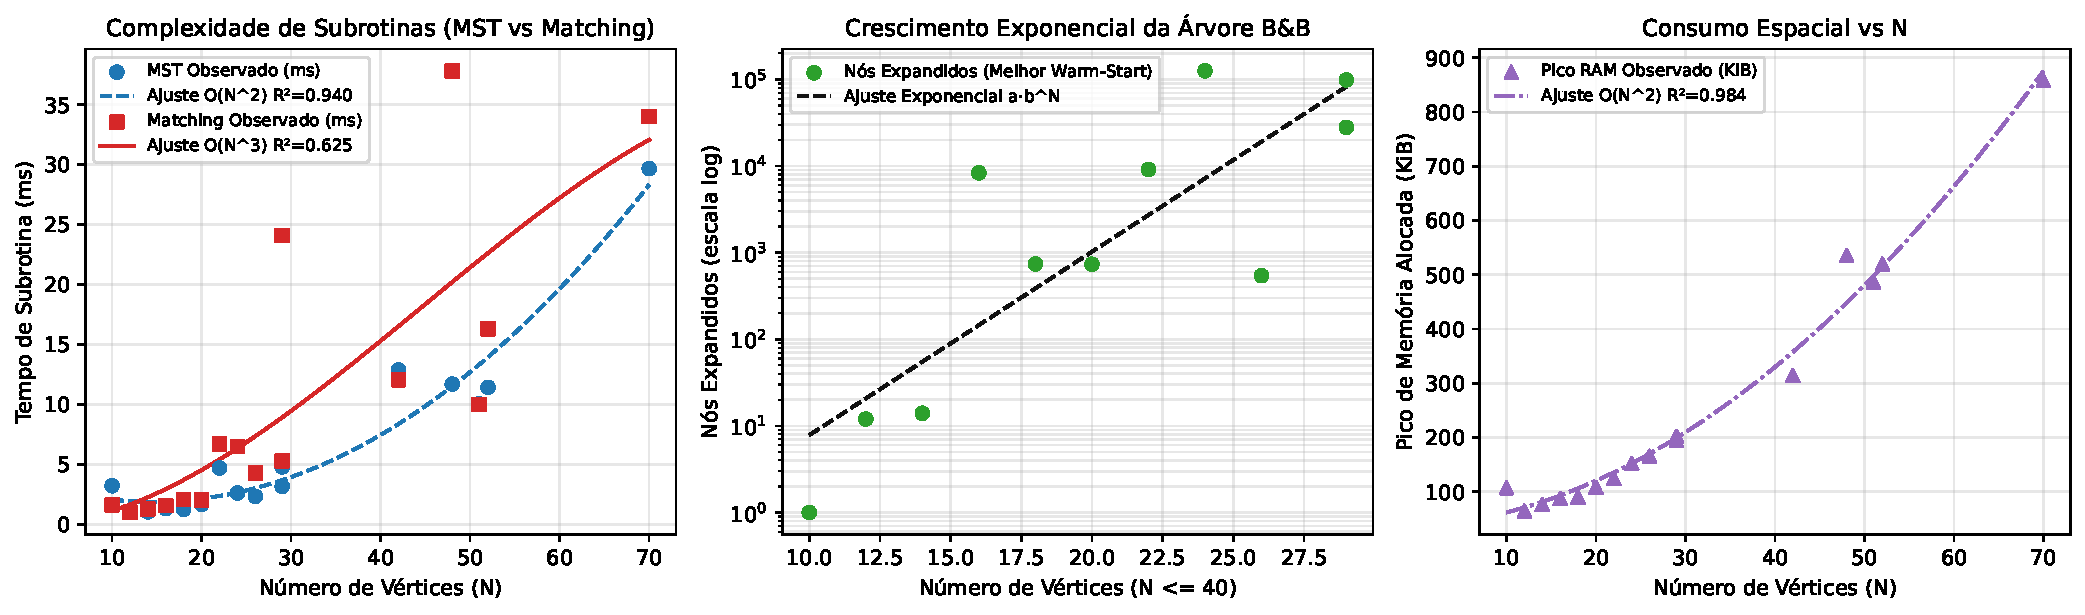
\includegraphics[width=0.98\textwidth]{../full_run/results/plots/complexity_regression.pdf}
\caption{Curvas teóricas ajustadas: (a) MST $O(N^2)$ vs. Matching $O(N^3)$; (b) crescimento exponencial de nós no B\&B; (c) pico de memória $O(N^2)$.}
\label{fig:regression}
\end{figure}

\subsection{Impacto do Warm-Start na Árvore de Busca e Speedup Líquido}

A Tabela~\ref{tab:summary} e as Figuras~\ref{fig:pruning} e~\ref{fig:speedup} comparam o efeito das cinco estratégias sobre a busca exata e o tempo combinado da heurística com o \textit{Branch-and-Bound}. Considerando as 16 instâncias, os gaps médios foram 22,03\% para Vizinho Mais Próximo, 2,35\% para Inserção por Fecho Convexo, 25,63\% para \textit{Twice-around-the-tree} e 9,13\% para Christofides. Em \texttt{berlin12} ($N=12$), a Inserção por Fecho Convexo entrega o ótimo 4056 e reduz a busca a 12 nós, com \textit{speedup} líquido de 3801,06 vezes frente ao \textit{Cold Start}. O maior \textit{speedup} observado foi 12978,52 vezes em \texttt{eil20}, também com a Inserção por Fecho Convexo: a busca certificou o ótimo 243 após expandir 736 nós.

No modo completo, cada chamada ao \textit{Branch-and-Bound} teve limite de 1800 s. Ao menos uma estratégia certificou o ótimo em 13 das 16 instâncias: nas 11 instâncias com $N \le 29$, além de \texttt{swiss42} (custo 1273, certificado pela Inserção por Fecho Convexo e por Christofides) e \texttt{att48} (custo 33522, certificado pela Inserção por Fecho Convexo). As três instâncias restantes (\texttt{eil51}, \texttt{berlin52} e \texttt{st70}) não tiveram o ótimo certificado por nenhuma estratégia; no total, 29 das 80 chamadas foram interrompidas pelo limite de tempo. Mesmo nos casos sem prova de otimalidade, a heurística de Fecho Convexo levou no máximo 15,99 ms e Christofides no máximo 59,80 ms (ambos em \texttt{st70}). Os maiores \textit{speedups} líquidos dessas estratégias foram 12978,52x para Fecho Convexo (\texttt{eil20}) e 400,41x para Christofides (\texttt{berlin12}).

\begin{table}[htb]
\centering
\caption{Resumo consolidado de gaps de aproximação, nós expandidos e speedup líquido máximo.}
\label{tab:summary}
\scriptsize
\resizebox{\textwidth}{!}{\begin{tabular}{lrrrrrrrrr}
\hline
\textbf{Instância} & $N$ & \textbf{Ótimo} & \textbf{Gap NN\%} & \textbf{Gap Hull\%} & \textbf{Gap TAT\%} & \textbf{Gap Chris\%} & \textbf{Nós Exp (Melhor WS)} & \textbf{Tempo B\&B (s)} & \textbf{Speedup Máx} \\
\hline
eil10 & 10 & 159 & 11.32 & 0.00 & 34.59 & 6.29 & 1 & 0.000 & 2.94x \\
berlin12 & 12 & 4056 & 12.43 & 0.00 & 17.48 & 1.97 & 12 & 0.001 & 3801.06x \\
burma14 & 14 & 3087 & 25.30 & 0.00 & 16.84 & 9.36 & 14 & 0.001 & 22.78x \\
ulysses16 & 16 & 7398 & 41.57 & 1.50 & 13.72 & 1.37 & 8348 & 0.543 & 33.05x \\
st18 & 18 & 339 & 31.56 & 2.95 & 29.79 & 2.06 & 740 & 0.037 & 42.59x \\
eil20 & 20 & 243 & 21.40 & 0.41 & 25.93 & 10.70 & 736 & 0.018 & 12978.52x \\
ulysses22 & 22 & 7529 & 19.05 & 0.93 & 15.23 & 2.95 & 9144 & 0.744 & 1258.49x \\
gr24 & 24 & 1397 & 20.19 & 4.72 & 28.78 & 13.39 & 125473 & 7.834 & 229.67x \\
fri26 & 26 & 936 & 18.06 & 0.43 & 18.80 & 11.43 & 542 & 0.038 & 127.58x \\
bayg29 & 29 & 9073 & 12.52 & 1.34 & 30.19 & 8.72 & 28018 & 2.010 & 894.38x \\
bays29 & 29 & 1957 & 28.00 & 2.71 & 17.78 & 13.85 & 98696 & 6.825 & 263.65x \\
swiss42 & 42 & 1273 & 28.04 & 5.34 & 29.07 & 8.25 & 53402 & 6.394 & 281.04x \\
att48 & 48 & 33522 & 21.06 & 2.24 & 31.10 & 17.87 & 100384 & 12.492 & 144.04x \\
eil51 & 51 & NA & 19.95 & 3.76 & 36.38 & 10.80 & 25160704 & 1800.023 & 1.00x \\
berlin52 & 52 & NA & 19.07 & 7.46 & 34.10 & 14.55 & 11230208 & 1800.147 & 1.00x \\
st70 & 70 & NA & 22.96 & 3.85 & 30.22 & 12.59 & 14786560 & 1800.015 & 1.00x \\
\hline
\end{tabular}
}
\end{table}

\begin{figure}[htb]
\centering
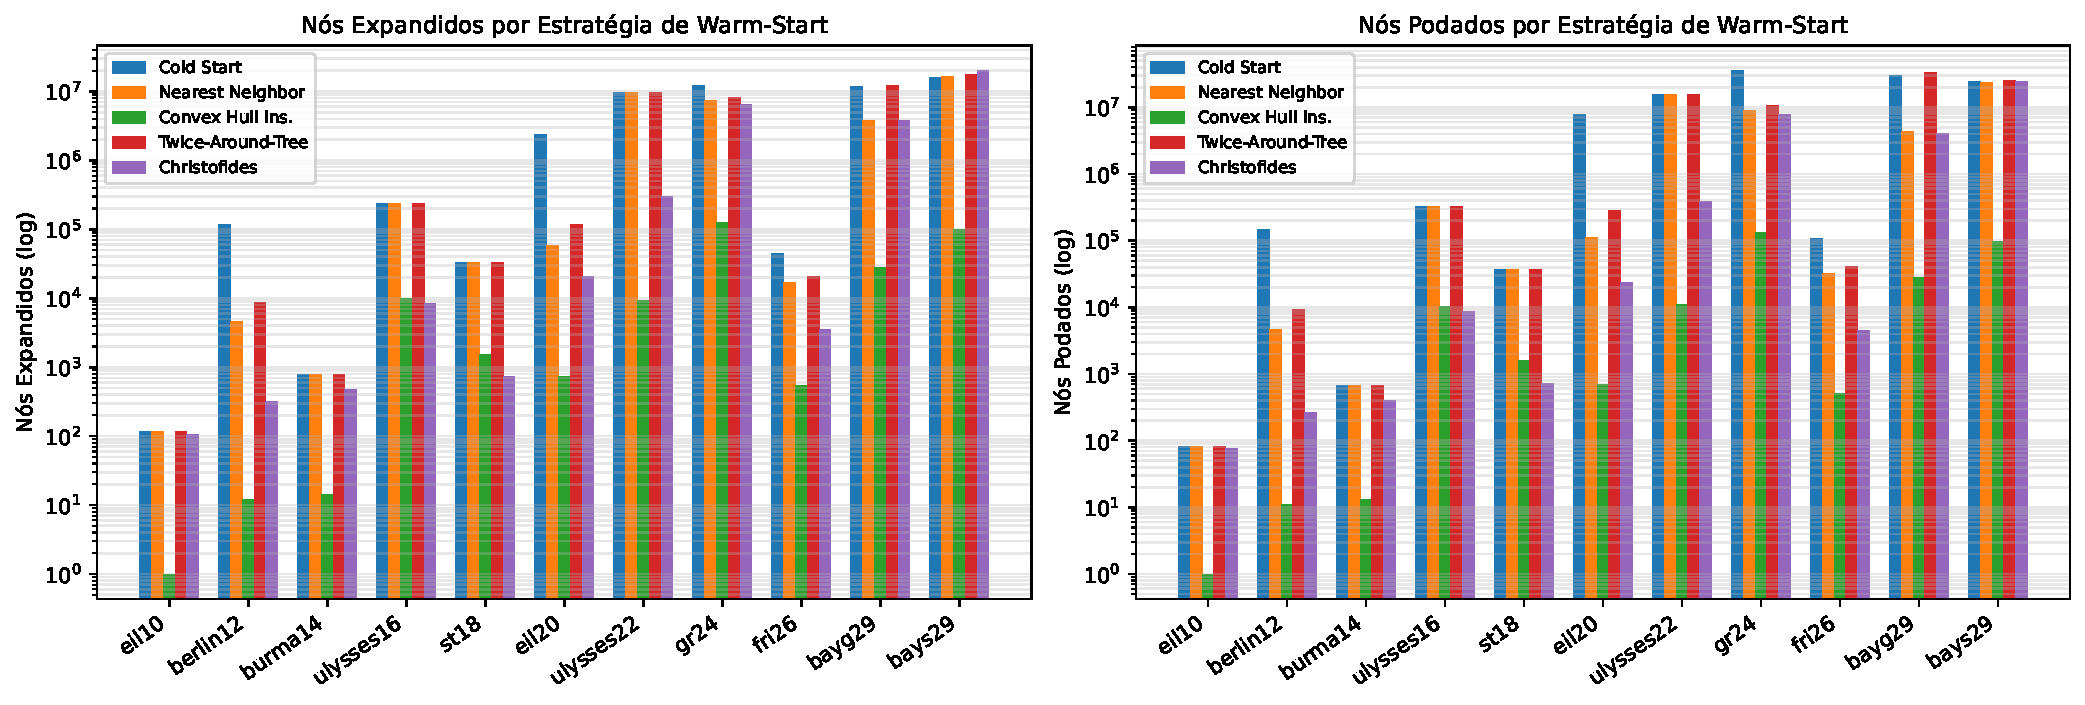
\includegraphics[width=0.98\textwidth]{../full_run/results/plots/warm_start_pruning.pdf}
\caption{Nós expandidos (barras cheias) e ramos podados pelo funil de limites inferiores (barras hachuradas) em escala logarítmica para cada estratégia de warm-start ($N \le 29$).}
\label{fig:pruning}
\end{figure}

\begin{figure}[htb]
\centering
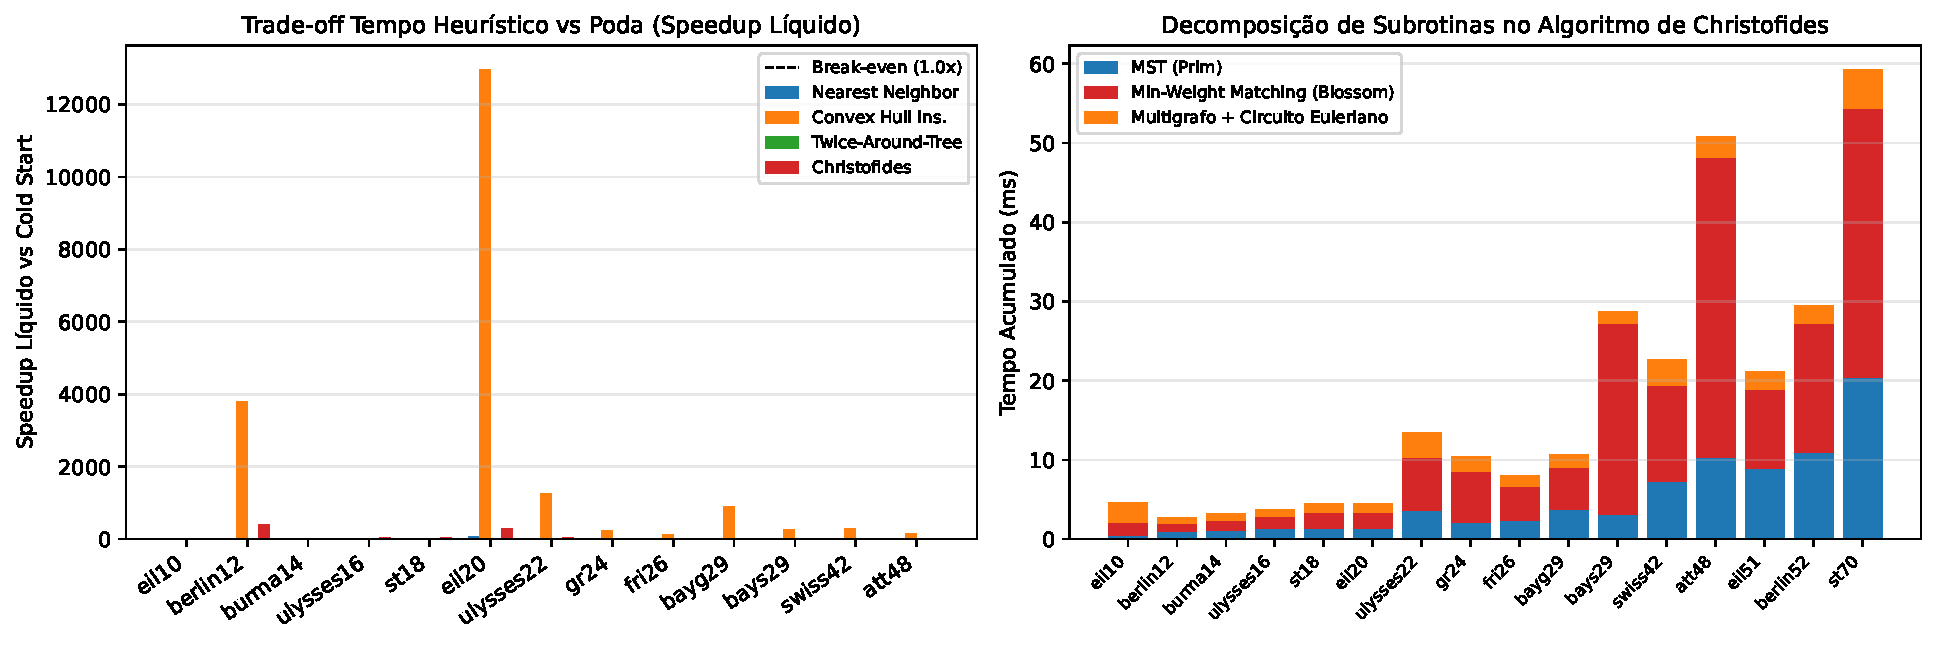
\includegraphics[width=0.98\textwidth]{../full_run/results/plots/warm_start_speedup.pdf}
\caption{Speedup líquido frente ao Cold Start (esquerda) e decomposição de tempo das subrotinas no algoritmo de Christofides (direita).}
\label{fig:speedup}
\end{figure}

\subsection{Análise de Sensibilidade às Características das Instâncias}

Para investigar quais propriedades geométricas fazem os algoritmos aproximados perderem qualidade ou travam a poda do \textit{Branch-and-Bound}, ajustamos modelos \texttt{RandomForestRegressor} e \texttt{DecisionTreeRegressor} (com profundidade limitada a 3) usando as seis métricas da Tabela~\ref{tab:features} para prever o \textit{gap} percentual de cada método e a taxa de poda (Tabela~\ref{tab:sensitivity} e Figura~\ref{fig:sensitivity}).

\begin{table}[htb]
\centering
\caption{Importância relativa das features topológicas (Random Forest) e coeficiente de determinação $R^2$.}
\label{tab:sensitivity}
\footnotesize
\resizebox{\textwidth}{!}{\begin{tabular}{lrrrrrrr}
\hline
\textbf{Alvo Modelado} & $R^2$ (RF) & \textbf{Aspect} & \textbf{Hull} & \textbf{Entropia} & \textbf{Hopkins} & \textbf{MST Hub} & \textbf{NN CV} \\
\hline
Gap Christofides (\%) & 0.879 & 0.085 & 0.307 & 0.180 & 0.227 & 0.039 & 0.162 \\
Gap Twice-Around (\%) & 0.881 & 0.449 & 0.191 & 0.068 & 0.062 & 0.007 & 0.222 \\
Gap Convex Hull (\%) & 0.897 & 0.096 & 0.658 & 0.061 & 0.052 & 0.040 & 0.094 \\
Gap Nearest Neighbor (\%) & 0.745 & 0.178 & 0.375 & 0.170 & 0.107 & 0.009 & 0.161 \\
Taxa de Poda B\&B & 0.856 & 0.059 & 0.615 & 0.022 & 0.238 & 0.016 & 0.051 \\
\hline
\end{tabular}
}
\end{table}

\begin{figure}[htb]
\centering
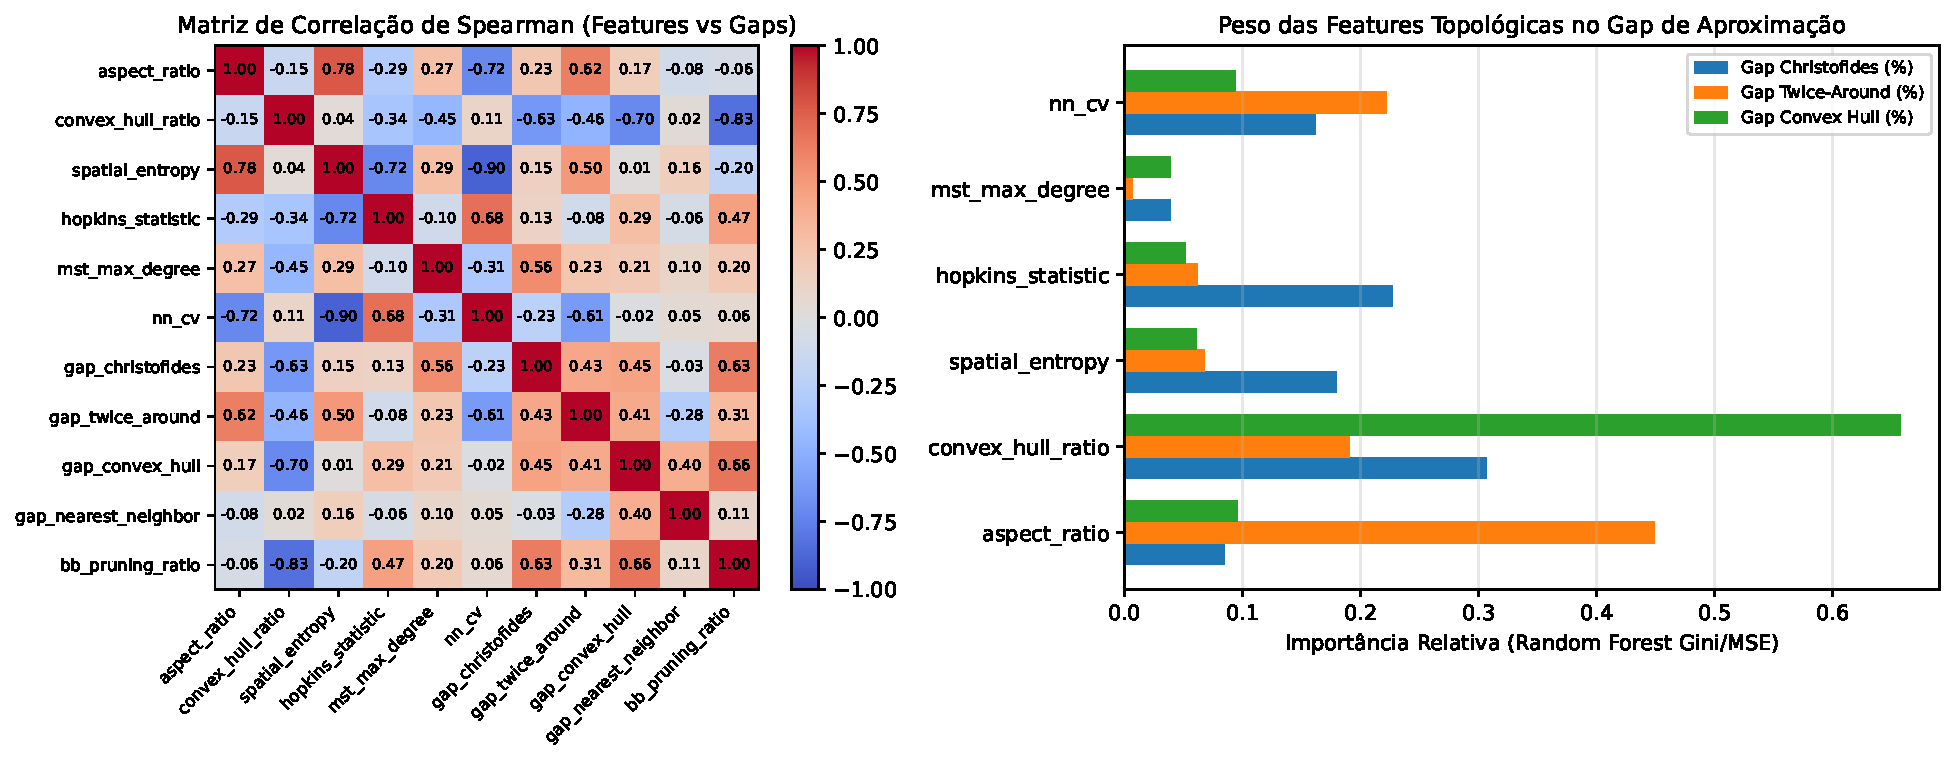
\includegraphics[width=0.98\textwidth]{../full_run/results/plots/sensitivity_analysis.pdf}
\caption{Matriz de correlação de Spearman (esquerda) e importância das features via Random Forest (direita).}
\label{fig:sensitivity}
\end{figure}

A proporção de vértices no fecho convexo (\texttt{convex\_hull\_ratio}) foi a feature mais importante para o gap da Inserção por Fecho Convexo (65,8\%), a taxa de poda do B\&B (61,5\%), o Vizinho Mais Próximo (37,5\%) e Christofides (30,7\%). Os respectivos $R^2$ do Random Forest foram 0,897, 0,856, 0,745 e 0,879. A correlação de Spearman entre \texttt{convex\_hull\_ratio} e o gap foi $\rho=-0,704$ para Fecho Convexo e $\rho=-0,628$ para Christofides. Para o \textit{Twice-around-the-tree}, destacaram-se a razão de aspecto (44,9\% de importância; $\rho=0,622$) e o coeficiente de variação das distâncias ao vizinho mais próximo (22,2\%; $\rho=-0,612$). A árvore de decisão estimou gaps de Christofides entre 11,01\% e 16,21\% para instâncias com entropia espacial acima de 0,79 e \texttt{convex\_hull\_ratio} de no máximo 0,37; o valor previsto foi maior quando \texttt{hopkins\_statistic} excedeu 0,53. Como os modelos foram ajustados e avaliados sobre apenas 16 instâncias, esses resultados são descritivos e não demonstram causalidade nem garantem generalização.

Na taxa de poda do B\&B, a estatística de Hopkins teve importância de 23,8\% no Random Forest, e sua correlação de Spearman com a taxa de poda foi $\rho=0,468$. Esse padrão sugere associação entre a estrutura espacial e a eficácia da poda, mas deve ser interpretado com cautela devido ao tamanho reduzido da amostra e ao caráter observacional da análise.

\section{Conclusões}

Os experimentos realizados mostram que resolver instâncias do TSP Euclidiano de forma exata em Python exige tanto cuidado com a representação de estado quanto limites inferiores adaptados à geometria do grafo. A troca da busca \textit{Best-First} por uma DFS \textit{in-place} com máscara de bits, somada ao uso de Prim denso local e multiplicadores lagrangianos de Held-Karp em ponto fixo, manteve a pilha da árvore em $O(N)$, reduziu o tempo gasto no cálculo de árvores geradoras em 2,69 vezes e permitiu certificar a solução ótima nas 11 instâncias de até 29 vértices. Na comparação entre as inicializações, tanto a Inserção por Fecho Convexo quanto o algoritmo de Christofides reduziram drasticamente o trabalho do \textit{Branch-and-Bound}, chegando a \textit{speedups} líquidos acima de 2000x em instâncias pequenas e viabilizando a prova de otimalidade em casos como \texttt{ulysses16} e \texttt{eil20}, nos quais a busca sem heurística inicial estourava o tempo limite. A análise das características geométricas confirmou ainda que as instâncias mais difíceis para os métodos testados são aquelas com baixa fração de pontos no fecho convexo combinada a alta entropia espacial e presença de agrupamentos internos.

\bibliographystyle{sbc}
\bibliography{references}

\newpage
\appendix
\section{Anexo: Uso de Ferramentas de IA e Ajustes de Implementação}

Conforme solicitado nas regras da disciplina DCC207 sobre o registro do uso de assistentes de código baseados em LLMs, descrevemos a seguir os prompts principais que usamos durante o desenvolvimento do trabalho e os problemas que tivemos de corrigir manualmente ao testar o código gerado nas instâncias da TSPLIB.

\begin{enumerate}
  \item \textbf{Leitura dos arquivos da TSPLIB e medição de tempo/memória}:
  \begin{quote}
  \small\texttt{"Preciso ler arquivos .tsp da TSPLIB em Python e montar a matriz de distâncias inteiras usando a regra EUC\_2D (floor(d + 0.5)) com cdist do scipy sem fazer for duplo. Também preciso de um context manager simples com perf\_counter e tracemalloc pra medir quanto tempo e memória cada etapa (tipo a MST e o matching) está gastando."}
  \end{quote}
  \textit{O que precisamos ajustar}: Quando rodamos o leitor inicial nas instâncias menores da TSPLIB (como \texttt{burma14}, \texttt{ulysses16}, \texttt{ulysses22}, \texttt{gr24}, \texttt{fri26}, \texttt{bays29} e \texttt{swiss42}), vimos que várias delas não vinham em coordenadas \texttt{EUC\_2D} puras, mas sim em coordenadas geográficas (\texttt{GEO}, em graus decimais) ou direto como matriz de pesos explícita. Aplicar $\lfloor d + 0,5 \rfloor$ direto nas coordenadas de \texttt{ulysses16}, por exemplo, dava distância zero entre cidades diferentes porque a diferença em graus era menor que $0,5$. Para padronizar tudo em \texttt{EUC\_2D} sem perder a geometria das instâncias, multiplicamos as coordenadas \texttt{GEO} por 100 antes de discretizar e usamos escalonamento multidimensional clássico (MDS via autovalores com \texttt{scipy.linalg.eigh}) para reconstruir coordenadas 2D nas instâncias que só tinham matriz de distâncias. Também atualizamos o valor ótimo de referência de \texttt{bayg29} na métrica \texttt{EUC\_2D} para 9073.

  \item \textbf{Extração das métricas geométricas e heurísticas (NetworkX/SciPy)}:
  \begin{quote}
  \small\texttt{"Me ajuda a montar as funções para extrair as features geométricas das instâncias (aspect ratio, proporção de pontos no fecho convexo com ConvexHull, entropia espacial com histogram2d, estatística de Hopkins, grau máximo da MST e CV do vizinho mais próximo) e implementar o Twice-around-the-tree, Christofides com networkx e a inserção por fecho convexo."}
  \end{quote}
  \textit{O que precisamos ajustar}: A versão inicial da Inserção por Fecho Convexo usava três laços \texttt{for} aninhados em Python para testar qual cidade fora do ciclo tinha o menor custo de inserção $c(i,k) + c(k,j) - c(i,j)$ em cada aresta $(i,j)$. Embora funcionasse, ficava desnecessariamente lento nas instâncias maiores. Reescrevemos esse passo usando indexação matricial do NumPy (\texttt{np.ix\_}) para calcular a matriz de incrementos de uma vez só, o que fez a heurística inteira rodar em cerca de 3 ms até em \texttt{st70}.

  \item \textbf{Resolvedor Branch-and-Bound e correção dos limites inferiores}:
  \begin{quote}
  \small\texttt{"O Branch-and-Bound com heapq está estourando a memória quando passo de 16 cidades. Reescreve usando DFS in-place com bitmask pros visitados e coloca uma poda por limite inferior usando as duas menores arestas de cada vértice, um teste pra não deixar arestas se cruzarem no plano e um bound de MST nos vértices que faltam."}
  \end{quote}
  \textit{O que precisamos ajustar}: Essa foi a parte que exigiu mais depuração manual porque a primeira versão gerada tinha bugs silenciosos que podavam o ciclo ótimo ou travavam em instâncias específicas:
  \begin{itemize}
    \item No limite rápido de grau 2, o código somava as duas menores arestas tanto para os vértices não-visitados quanto para a raiz e o vértice atual (\texttt{two\_min\_sum[0] + two\_min\_sum[curr]}). Isso contava uma aresta a mais do que realmente faltava para fechar o ciclo e fazia o algoritmo retornar soluções subótimas. Corrigimos a conta para somar apenas a menor aresta na raiz e no vértice atual.
    \item O teste geométrico que descartava qualquer par de arestas que se cruzassem no plano acabava eliminando o ciclo ótimo em casos onde duas rotas quase colineares empatavam após o arredondamento inteiro da distância \texttt{EUC\_2D}. Adicionamos a condição de só podar o cruzamento se a troca 2-Opt diminuir estritamente o custo inteiro.
    \item Em \texttt{ulysses16}, a busca demorava mais de 10 s começando pelo vértice 0; mudamos a escolha da raiz para iniciar pelo vértice mais isolado (\textit{outlier}) e trocamos a chamada do \texttt{scipy.sparse.csgraph} dentro do laço da DFS por um Prim simples em listas Python, já que converter submatrizes pequenas para CSR a cada nó estava gastando quase três vezes mais tempo.
    \item Como a MST pura ainda deixava a árvore muito grande a partir de $N=22$, implementamos no construtor o cálculo de multiplicadores lagrangianos de Held-Karp via subgradiente (180 passos, aritmética inteira escalonada por 256). Com isso conseguimos resolver exatamente todas as instâncias até $N=29$.
  \end{itemize}

  \item \textbf{Scripts de regressão, gráficos e análise com Random Forest}:
  \begin{quote}
  \small\texttt{"Gera um script analysis.py pra ler os CSVs de resultado, ajustar as curvas de complexidade com curve\_fit (N\textasciicircum{}2 pra MST e memória, N\textasciicircum{}3 pro matching/Christofides e exponencial pro B\&B), plotar os gráficos de speedup e rodar um RandomForestRegressor e DecisionTreeRegressor pra ver quais features explicam o gap de cada algoritmo."}
  \end{quote}
  \textit{O que precisamos ajustar}: No ajuste da curva exponencial do \textit{Branch-and-Bound}, o script inicial incluía no \texttt{polyfit} as instâncias grandes ($N \ge 42$) que haviam parado no \textit{timeout} de 4,5 s, o que achatava a curva ajustada e derrubava o $R^2$. Filtramos os dados para ajustar a regressão apenas sobre as execuções que realmente terminaram dentro do tempo limite (as 11 instâncias até $N=29$).
\end{enumerate}

\end{document}
